\documentclass{beamer}

\usepackage[utf8]{inputenc}
\usepackage[english]{babel}
\usepackage[T1]{fontenc}
\usepackage{lmodern}
\usepackage{adjustbox}
\usepackage{graphicx}
\usepackage{commath}
\usepackage{amsmath,amssymb,amsthm}
\usepackage{tikz}
\usepackage{pgffor}
\usepackage[lined]{algorithm2e}
\usepackage[
  style=numeric,
  natbib=true,
  sortcites=true,
  block=space,
  citestyle=verbose]{biblatex}
\bibliography{biblio}%
\usetheme{Singapore}
\newlength{\mylen}
\resetcounteronoverlays{compt}
\AtBeginSection[]
{
  \begin{frame}<beamer>
    \frametitle{Overview}
    \tableofcontents[currentsection]
  \end{frame}
}
\addtobeamertemplate{navigation symbols}{}{%
    \usebeamerfont{footline}%
    \usebeamercolor[fg]{footline}%
    \hspace{1em}%
    \insertframenumber/\inserttotalframenumber
}
\begin{document}

\title{Integrating lexical constraints and background knowledge to $K$-Means with Deep Learning}
\author{Maxence Grand \\                                                   
        Supervised by : Thibaut Thonet \and \'Eric Gaussier  \and Marc Tommasi \and Aur\'elien Bellet \and  Maziar Moradi Fard} 
\institute{Laboratoire d'Informatique de Grenoble, Team AMA}
\date{\today}

\maketitle

\begin{frame}{Overview}
\tableofcontents
\end{frame}
\section{Introduction}

\begin{frame}
\frametitle{$K$-Means}
Given a corpus C, where each document X is a 
N-dimensional real vector, k-means clustering aims to partition the n 
documents into K $S_k$ clusters represented by centroids 
R = {$r_1, r_2, ..., r_K$}. :
Formally, the objective is to minimize :
$$
\sum_{k =1 }^K \sum_{X \in S_k} ||X - r_k||_2^2
$$
\end{frame}

\foreach \n in {0,...,7}{
  \begin{frame}
    \frametitle{$K$-Means}
  \begin{figure}[!h]
    \centering
    \includegraphics[scale=0.45]{kmeans/\n test.png}
  \end{figure}
  \end{frame}
}

\begin{frame}
  \frametitle{Lexical Constraints}
  \pause
  \begin{itemize}
    \setlength\itemsep{2em}
  \item Set of keywords \pause
  \item Bias clustering
  \end{itemize}
\end{frame}
\begin{frame}
\frametitle{Background Knowledge}
\begin{itemize}
\pause
\item \textbf{Must-link} constraint $ML$ : $(X, X') \in ML \implies $ X and X' are in the
  same cluster.\pause
\item \textbf{Cannot-link} constraint $CL$ : $(X, X') \in CL \implies $ X and X' are in
  different cluster.
\end{itemize}
\end{frame}

\begin{frame}
  \frametitle{Background Knowledge - COP$K$-Means}
  \begin{columns}[T] % align columns
    \setlength{\mylen}{0.5\textwidth}
    \begin{column}{\mylen}
      \scalebox{.6}{                        %new code
        \begin{algorithm}[H]
          \SetKwInOut{Input}{input}
          \SetKwInOut{Output}{output}
          \Input{Corpus C, must-link constraints $ML \subseteq C x C$,
            cannot-link constraints $CL \subseteq C x C$}
          \Output{Clusters $S_1, S_2, ..., S_k$}
          Let $S_1, S_2 , ..., S_k$ be the initial clusters\\
          \Repeat{Convergence}{
            \ForEach{$X_i \in C$}{
              Assign $X_i$ to closest $S_j$ such that Violate-Constraints($X_i, C_j, CL,
              ML$) is false.\\
              \If{No such clusters exists}{
                return \{\}\\
              }
            }
            \ForEach{Clusters $S_i$}{
              Update centroids.\\
            }
          }
          \Return{$S_1, S_2, ..., S_k$}
          \caption{\label{algo:cop}COP-Kmeans}
        \end{algorithm}  
      }
    \end{column}%
    \hfill%
    \begin{column}{\dimexpr\textwidth-\mylen}
      \scalebox{.7}{                        %new code
        \begin{algorithm}[H]
          \SetKwInOut{Input}{input}
          \SetKwInOut{Output}{output}
          \Input{Ducument X, Clusters S, must-link constraints $ML \subseteq C x C$,
            cannot-link constraints $CL \subseteq C x C$}
          \Output{True if constraints are violate, False otherwise}
          \ForEach{($X, X' \in ML$)}{
            \If{$X' \in S$}{
              \Return{True}
            }
          }
          \ForEach{($X, X' \in CL$)}{
            \If{$X' \in S$}{
              \Return{True}
            }
          }
          \Return{False}
          \caption{\label{algo:vio}Violate-Constraints}
        \end{algorithm}
        
      }
    \end{column}%
  \end{columns}
\footnote{Wagstaff et al}
\end{frame}

\begin{frame}
\frametitle{Background Knowledge - NNClustering}
\begin{equation*}
  P = f_{NN}(X_p), ~ Q = f_{NN}(X_q)
\end{equation*}
\pause
\begin{equation*}
  KL(P||Q) = \sum_i^k P_ilog\frac{P_i}{Q_i}
\end{equation*}
\pause
\begin{equation*}
  I_s = \left\{
\begin{array}{ll}
  1 & \mbox{if ($X_p, X_q$) $\in$ ML }\\
  0 & \mbox{Otherwise.}
\end{array}
\right.
\end{equation*}
%
\begin{equation*}
  I_{ds} = \left\{
\begin{array}{ll}
  1 & \mbox{if ($X_p, X_q$) $\in$ CL}\\
  0 & \mbox{Otherwise.}
\end{array}
\right.
\end{equation*}
\begin{equation*}
  Loss(P || Q) = I_s(X_p, X_q)KL(P || Q) + I_{ds}(X_p, X_q)max(0,
  \eta-KL(P||Q))
\end{equation*}
\begin{equation*}
  L(P,Q) = Loss(P || Q) + Loss(Q || P)
\end{equation*}
\footnote{Hsu et al}
\end{frame}

%Bas de page pour COP-KMeans et NNclust
\begin{frame}
\begin{itemize}
  \setlength\itemsep{1em}
\item Encode Function $h_{\theta}(X) = g(X; \theta)$
\item Decode Function $f(Y; \theta)$
\item $L_{rec}(X, \theta) = || X - f(h_{\theta}(X); \theta)||_2^2$
\end{itemize}
  \frametitle{Auto-Encoder}
  \begin{figure}[!h]
    \centering
    \fbox{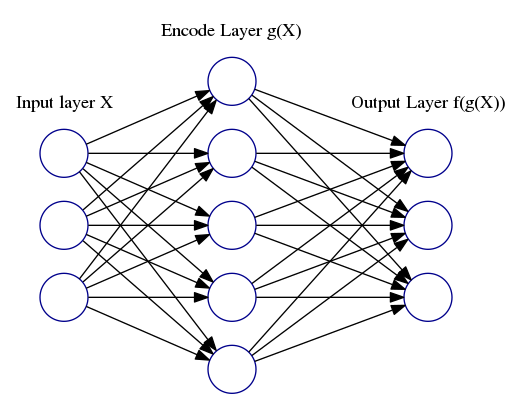
\includegraphics[scale=0.2]{autoencoder.png}}
    \label{fig:AE}
  \end{figure}
\end{frame}

\section{Proposed Method}

%Remplacer \Omega par L_{const}
\begin{frame}
\frametitle{The Idea}
Learn a latent space taking into account lexical constraints and
background knowledge.
\end{frame}

\begin{frame}
\frametitle{Lexical Constraints}
\begin{equation*}
KW = \begin{pmatrix} kw_1 & kw_2 & ... & kw_{N_{kw}-1} & kw_{N_{kw}}
\end {pmatrix}
\end{equation*}
\pause
Introducing $X'$ such that
\begin{equation*}
\forall_{i=1,2,..,N}X_i' = \left\{
\begin{array}{ll}
  X_i & \mbox{if } i \in KW \\
  0 & \mbox{Otherwise.}
\end{array}
\right.
\end{equation*}
\pause
\begin{equation*}\label{eq:omega1}
  \omega_{KW} = \sum_{X \in C} || h_{\theta}(X) - h_{\theta}(X')||_2^2
\end{equation*}
\end{frame}

\begin{frame}
\frametitle{Pairwise Constraints}
\pause
\begin{itemize}
\item Must-Link : $$\omega_{ML} = \sum_{\forall{(X_i,X_j)\in ML}} || h_{\theta}(X_i) - h_{\theta}(X_j) ||_2^2$$ \pause
\item Cannot-Link : $$\omega_{CL} = \sum_{\forall{(X_i,X_j)\in CL}} max(0,
  \eta - || h_{\theta}(X_i) - h_{\theta}(X_j) ||_2^2)$$
\end{itemize}
\end{frame}

\begin{frame}
  \frametitle{Deep $K$-Means }
\begin{equation*}
  L_{Clust}(C,\beta;\theta,R) = \sum_{X \in C} ||h_\theta(X)-c(h_\theta(X); R)||_2^2
\end{equation*}
\begin{equation*}
  c(h_\theta(X); R) = argmin_{r \in R}||h_\theta(X) - r||_2^2
\end{equation*}
\end{frame}

\begin{frame}
  \frametitle{Deep $K$-Means }
\begin{equation*}
L_{Clust}(C, K, \beta; \theta, R) = \sum_{X \in C} \sum_{k=1}^K ||h_{\theta}(X) - r_k||_2^2 G_{k, F}(h_{\theta}(X), \beta; R)
\end{equation*}
\begin{equation*}
G_{k, F}(h_{\theta}(X), \beta; R) = \frac{e^{-\beta ||g(X, \theta) - r_k||_2^2}}
{\sum_{k' = 1}^K e^{-\beta ||g(X, \theta) - r_k||_2^2}}
\end{equation*}
\end{frame}

\begin{frame}
\frametitle{Final Loss}
\begin{equation*}
  L_{const}(C, KW;\theta) = \alpha_0\omega_{KW} + \alpha_1\omega_{CL} + \alpha_2\omega_{ML}  
\end{equation*}
\pause
\begin{equation*}
  L_{rec}(C, \theta) = \sum_{X \in C}(||X - f(h_\theta(X))||_2^2
\end{equation*}
\pause
\begin{equation*}
  L(C,KW; \theta) = L_{rec}(C, \theta) + L_{const}(C, KW;\theta) + \lambda.L_{Clust}(C, K, \beta; \theta, R)   
\end{equation*}
\end{frame}

\section{Experiment}

\begin{frame}
  \frametitle{Data}
  \begin{itemize}
    \setlength\itemsep{2em}
  \item 20 newsgroups
  \item RCV1 
  \end{itemize}
\end{frame}

\begin{frame}
\frametitle{Generate Lexical Constraints}
\scalebox{.7}{
\begin{algorithm}[H]
  \SetKwInOut{Input}{input}
  \SetKwInOut{Output}{output}
  \Input{Corpus C, The number of keywords per classes $P$}
  \Output{KW}
  $KW \gets \{\}$\\
  \ForEach{Class $c_i \in C$}{
    $rank_i \gets [0 ... 0]$\\
    \ForEach{Document $X \in c_i$}{
      \ForEach{Word $w \in X$}{
        $rank_{i,w} \gets rank_{i,w} + TFIDF(w,X, C)$\\
      }
    }
  }
  \ForEach{Class $c_i, c_j \in C$}{
    \If{$c_i \neq c_j$}{
      $rank_i \gets rank_i - rank_j$\\
    }
  }
  \ForEach{Class $c_i \in C$}{
    $KW \gets KW \cup \{\{w_1, w_2 ... w_P\} : \not\exists (v_1, v_2) | v_1 \not\in 
    \{w_1, w_2 ... w_P\}, v_2 \in \{w_1, w_2 ... w_P\}, rank_{i,v_1} \ge rank_{i,v_2}\}$\\
  }
  \Return{KW}
  \caption{\label{algo:gen_kw}Extract Keywords}
\end{algorithm}
}
\end{frame}

\begin{frame}
\frametitle{Metric}
\begin{itemize}
\item NMI
\item Accuracy
\item Adjusted Rand Index
\end{itemize}
\end{frame}

\begin{frame}
\frametitle{Baseline Algorithm}
Deep $K$-Means algorithm.
\end{frame}

\begin{frame}
\frametitle{Architecture}
\begin{figure}[!h]
  \centering
  \fbox{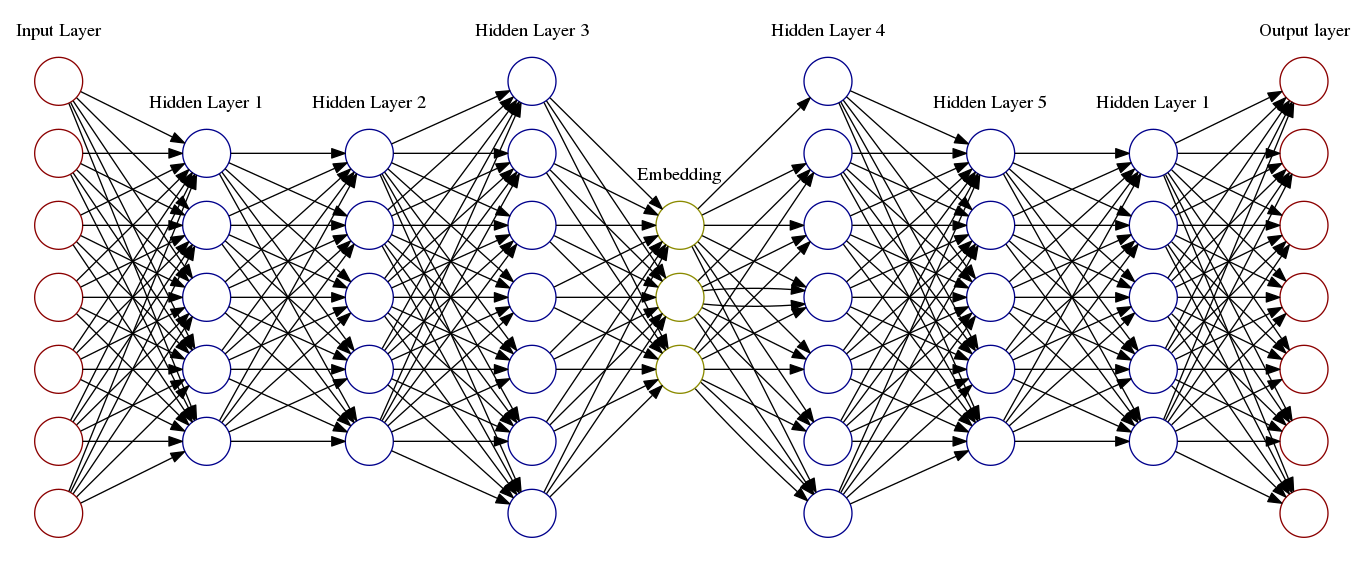
\includegraphics[scale=0.2]{archi.png}}
  \caption{\label{fig:archi}Architecture}
\end{figure}
\end{frame}

\begin{frame}
\frametitle{Hyperparameters}
\begin{equation*}
L(C,KW, K; \theta) = L_{rec}(C, \theta) + L_{const}(C, KW;\theta) + \lambda.L_{Clust}(C, K, \beta; \theta, R)
\end{equation*}
with
\begin{equation*}
L_{const}(C, KW;\theta) = \alpha_0\omega_{KW} + \alpha_1\omega_{CL} + \alpha_2\omega_{ML}
\end{equation*}
\begin{table}[!h]
\centering
\resizebox{\textwidth}{!}{%Details sur le line search
  \begin{tabular}{| l | l | l | l |}
    \hline
               & 20NEWS Without noise & 20NEWS With noise & RCV1 Without noise  \\ \hline
    $\lambda$  & $10^{-1}$            & $10^{-1}$         & $10^{-2}$           \\ \hline
    $\alpha_0$ & $10^{-2}$            & $5.10^{-3}$       & $10^{-1}$           \\ \hline
    $\alpha_1$ & 0                    & 0                 & 0                   \\ \hline
    $\alpha_2$ & 0                    & 0                 & 0                   \\ \hline
    $\eta$     & 0                    & 0                 & 0                   \\ \hline
  \end{tabular}
}
\end{table}
\end{frame}

\begin{frame}
\frametitle{Results}
\begin{table}[!h]
\resizebox{\textwidth}{!}{%Inverser lignes/colonnes
  \begin{tabular}{|l|l|l|l|l|l|l|}
    \hline
    & \multicolumn{3}{|c|}{DKM} & \multicolumn{3}{|c|}{CDKM}\\
    & ACC         &ARI          & NMI         & ACC         & ARI          &NMI  \\ \hline
20NEWS without noise   &$51.7\pm 1.9$&$33.6\pm 1.1$&$47.1\pm 0.9$&\boldmath$53.4\pm 2.2$&\boldmath$35.4\pm 1.2$ &\boldmath$47.4\pm 0.9$ \\ \hline
20NEWS with noise   &$42.8\pm 3.3$&$20.7\pm 1.9$&$28.3\pm 0.8$&\boldmath$45.3\pm 3$  &\boldmath$23.23\pm 2.3$&\boldmath$30.0\pm 1.7$ \\ \hline
RCV1 without noise   &$55.3\pm 3.4$&$24.1\pm 5.5$&$30.5\pm 5.3$&\boldmath$62.7\pm 5$  &\boldmath$31.7\pm 3.9$ &\boldmath$37.2\pm 4$   \\ \hline
  \end{tabular}
}
\end{table}
\end{frame}

\section{Conclusion \& Future Works}

\begin{frame}
  \frametitle{Conclusion \& Future Works}
\begin{itemize}
\item We have presented and tested in this study an approach to integrate lexical constraints to $K$-Means algorithm. \pause 
\item Future Works
\begin{itemize}
\item Test pairwise constraints
\item More baseline Algorithm
\begin{itemize}
\item COP$K$-Means
\item Deep COP$K$-Means
\end{itemize}
\item Robustness
\begin{itemize}
\item Change number of keywords
\item Change number of cluster
\end{itemize}
\end{itemize}
\end{itemize}
\end{frame}

\begin{frame}
Any Questions ?
\end{frame}

\begin{frame}
\frametitle{$G_{F,k}$ \& $\beta$}
\begin{equation*}
G_{k, F}(h_{\theta}(X), \beta; R) = \frac{e^{-\beta ||h_\theta(X) - r_k||_2^2}}
{\sum_{k' = 1}^K e^{-\beta ||g(X, \theta) - r_k||_2^2}}
\end{equation*}
\begin{equation*}
  \lim\limits_{\beta \rightarrow \beta_0}G_{k, F}(h_\theta(X), \beta; R) = \left\{
\begin{array}{ll}
  1 & \mbox{if }r_k = c(h_\theta(X); R)\\
  0 & \mbox{Otherwise.}
\end{array}
\right.
\end{equation*}
where $\beta$ play the role of an inverse temperature.
\end{frame}

\begin{frame}
\frametitle{Stochastic gradient descent (SGD)}
\begin{equation*}
  (\theta, R) \gets (\theta, R) - \epsilon \frac{1}{|\widetilde{C}|}
  \nabla_{(\theta, R)} L(C, \beta; \theta, R)
\end{equation*}
where $\widetilde{C}$ is a random mini batch of C, and $\epsilon$ the
learning rate.
\end{frame}
\begin{frame}
\frametitle{Training dkm}
\scalebox{0.7}{
\begin{algorithm}[H]
  \SetKwInOut{Input}{input}
  \SetKwInOut{Output}{output}
  \Input{Corpus C , number of clusters K, balancing parameter $\lambda$,
    scheme for $\beta$, number of epochs T ,
    number of minibatches MB , learning rate $\epsilon$}
  \Output{Auto-Encoder parameter $\theta$, cluster representative R}
  Initialise $\theta$ and $r_k$, $1 \leq k \leq K$ (randomly or through 
  pretraining)\\
  \ForEach{$\beta = m_\beta : M_\beta$}{
    \ForEach{t = 1 : T}{
      \ForEach{n = 1 : MB}{
        Draw minibatch $\widetilde{C} \subseteq  C$\\
        Update ($\theta, R$) using SGD
      } 
    }  
  }
\end{algorithm}
}
\end{frame}

\begin{frame}
\frametitle{Deep COP$K$-Means}
\begin{equation*}
  L( C, KW, K; \theta) = L_{rec}(C, \theta) + \omega_{KW} + \lambda.L_{Clust}(X, K, \beta;\theta, R)
\end{equation*}
\end{frame}

\begin{frame}
\frametitle{Metric - NMI}
The NMI Metric is defined as follows
$$NMI(S,C) = \frac{I(S,C)}{[H(S)+H(C)]/2}$$ 
with
$I(S,C) =\sum_k \sum_f\frac{|s_k \cap c_f|}{N}log\frac{N|s_k \cap c_f|}{|s_k| |c_f|}$
and
$H(S) = -\sum_k\frac{|s_k|}{N}log\frac{N|s_k|}{|s_k|}$
\end{frame}

\begin{frame}
\frametitle{Metric - Accuracy}
The Accuracy is the proportion of true results among the total
  number of cases examined. The Accuracy metric is defined as follows :
$$
ACC(S,C) = \frac{1}{N}\sum_k {max}_j|s_k \cap c_j|
$$
\end{frame}

\begin{frame}
\frametitle{Metric - Adjusted Rand Index}
Let a be the number of pairs of document in C
  that are in the same cluster in the predicted partition and in the
  same cluster in the real partition, and b be the number of pairs of
  document in C that are in different clusters in predicted partition
  and in different cluster in real partition.
  The Adjusted Rand index is defined as follows :
  $$ARI = \frac{a+b}{\binom{N}{2}}$$
\end{frame}
\end{document}
